\PassOptionsToPackage{xetex}{xcolor}
\PassOptionsToPackage{xetex}{graphicx}
\documentclass[a4paper,landscape,headrule,footrule,xetex]{foils}

%%
%%%  Macros
%%%
\newcommand{\logo}{~}
\MyLogo{HG2052 (2020)}
%\newcommand{\Story}{\SHA{HOUN}{The Hound of the Baskervilles}}

\newcommand{\header}[3]{%
\title{\vspace*{-2ex} \Large HG2052
\\\large  Language, Technology and the Internet
\\[2ex] \Large  \emp{#2}}
\author{\blu{Francis Bond}   \\ 
\normalsize  \textbf{Division of Linguistics and Multilingual Studies}\\
\normalsize  \url{http://www3.ntu.edu.sg/home/fcbond/}\\
\normalsize  \texttt{bond@ieee.org}}
\MyLogo{HG2052 (2020)}
\date{#1}
\renewcommand{\logo}{#2}
 \hypersetup{
   pdfinfo={
     Author={Francis Bond},
     Title={#1: #2},
     Subject={HG2052: Language, Technology and the Internet},
     Keywords={Language, Technology, Internet},
     License={CC BY 4.0}
   }
 %  pdfcopyright={Copyright © Francis Bond. Creative Commons 4.0 Attribution License.}
 %  pdflicenseurl={http://creativecommons.org/licenses/by/4.0/}
 }
}


%%
%% Multilingual Stuff
%%
\usepackage[a4paper,landscape,margin=25mm]{geometry}

\usepackage{fontenc}
\usepackage{polyglossia}
\setmainlanguage{english}
\setmainfont{TeX Gyre Pagella}
%\setmainfont{Linux Libertine}
%\setmainfont{Charis SIL}
\newfontfamily{\ipafont}{Gentium}
\newcommand{\ipa}[1]{{\ipafont\selectfont #1}}
\usepackage{xeCJK}

\setCJKmainfont{Noto Sans CJK SC}
\setCJKsansfont{Noto Sans CJK SC}
%\setCJKttfont{Noto Sans CJK SC}
%\setCJKmainfont{WenQuanYi Micro Hei}
%\clearpage
%\setCJKmainfont{AR PL SungtiL GB}

\usepackage[xetex]{xcolor}
\usepackage[xetex]{graphicx}
\newcommand{\blu}[1]{\textcolor{blue}{#1}}
\newcommand{\grn}[1]{\textcolor{green}{#1}}
\newcommand{\hide}[1]{\textcolor{white}{#1}}
\newcommand{\emp}[1]{\textcolor{red}{#1}}
\newcommand{\txx}[1]{\textbf{\textcolor{blue}{#1}}}
\newcommand{\lex}[1]{\textbf{\mtcitestyle{#1}}}

\usepackage{pifont}
\renewcommand{\labelitemi}{\textcolor{violet}{\ding{227}}}
\renewcommand{\labelitemii}{\textcolor{purple}{\ding{226}}}

\newcommand{\subhead}[1]{\noindent\textbf{#1}\\[5mm]}

\newcommand{\Bad}{\emp{\raisebox{0.15ex}{\ensuremath{\mathbf{\otimes}}}}}
\newcommand{\bad}{*}

\newcommand{\com}[1]{\hfill \textnormal{(\emp{#1})}}%
\newcommand{\cxm}[1]{\hfill \textnormal{(\txx{#1})}}%
\newcommand{\cmm}[1]{\hfill \textnormal{(#1)}}%
\usepackage{amssymb}
\usepackage{relsize,xspace}
\newcommand{\into}{\ensuremath{\rightarrow}\xspace}
\newcommand{\ent}{\ensuremath{\Rightarrow}\xspace}
\newcommand{\nent}{\ensuremath{\not\Rightarrow}\xspace}
\newcommand{\tot}{\ensuremath{\leftrightarrow}\xspace}
\usepackage{url}
\usepackage[hidelinks]{hyperref}
\hypersetup{
     colorlinks,
     linkcolor={blue!50!black},
     citecolor={red!50!black},
     urlcolor={blue!80!black}
}
%\usepackage{hyperxmp}
\usepackage{url}
\newcommand{\lurl}[1]{\MyLogo{\url{#1}}}

\usepackage{mygb4e}
\let\eachwordone=\itshape
\newcommand{\lx}[1]{\textbf{\textit{#1}}}
\newcommand{\ix}{\ex\it}

\newcommand{\cen}[2]{\multicolumn{#1}{c}{#2}}
%\usepackage{times}
%\usepackage{nttfoilhead}
\newcommand{\myslide}[1]{%
\foilhead[-25mm]{\raisebox{12mm}[0mm]{\emp{#1}}}%
\leftheader{}%
\MyLogo{\logo}}

\newcommand{\mytask}[1]{%
\foilhead[-25mm]{\raisebox{12mm}[0mm]{\emp{#1}}}
\leftheader{🔍 Hi}%
\MyLogo{\logo}}

\newcommand{\myslider}[1]{\rotatefoilhead[-25mm]{\raisebox{12mm}[0mm]{\emp{#1}}}}
%\newcommand{\myslider}[1]{\rotatefoilhead{\raisebox{-8mm}{\emp{#1}}}}

\newcommand{\section}[1]{\myslide{}{\begin{center}\Huge \emp{#1}\end{center}}}

\usepackage{tcolorbox}
% \newcommand{\task}{\marginpar{\raisebox{-1ex}{\large
%       \tcbox[colframe=red,colback=white,arc=3pt]{\textbf{?}}}}}
% \newcommand{\task}{\marginpar{\raisebox{-1ex}{
%       \hspace{-0.5em}\tcbox[colframe=red,colback=white,arc=3pt]{%
%         \includegraphics[width=1.5em]{pics/detective}}}}}
\newcommand{\task}{\marginpar{\raisebox{-2ex}{
      \hspace{-0.5em}\reflectbox{\includegraphics[width=2em]{pics/detective}}}}}

\usepackage[lyons,j,e,k]{mtg2e}
\renewcommand{\mtcitestyle}[1]{\textcolor{teal}{\textsl{#1}}}
%\renewcommand{\mtcitestyle}[1]{\textsl{#1}}
\newcommand{\chn}{\mtciteform}
\newcommand{\cmn}{\mtciteform}
\newcommand{\iz}[1]{\textup{\texttt{\textcolor{blue}{\textbf{#1}}}}}
\newcommand{\con}[1]{\textsc{#1}}
\newcommand{\gm}{\textsc}
\newcommand{\cmp}[1]{{[\textsc{#1}]}}
\newcommand{\sr}[1]{\ensuremath{\langle}#1\ensuremath{\rangle}}
\usepackage[normalem]{ulem}
\newcommand{\ul}{\uline}
\newcommand{\uul}{\uuline}
\newcommand{\wl}{\uwave}
\newcommand{\vs}{\ensuremath{\Leftrightarrow}~}
%%%
%%% Bibliography
%%%
\usepackage{natbib}
%\usepackage{url}
\usepackage{bibentry}


%%% From Tim
\newcommand{\WMngram}[1][]{$n$-gram#1\xspace}
\newcommand{\infers}{$\rightarrow$\xspace}



\usepackage{rtrees,qtree}
\renewcommand{\lf}[1]{\br{#1}{}}
\usepackage{avm}
%\avmoptions{topleft,center}
\newcommand{\ft}[1]{\textsc{#1}}
\newcommand{\val}[1]{\textit{#1}}
\newcommand{\typ}[1]{\textit{#1}}
\avmfont{\sc}
%\avmvalfont{\sc}
\renewcommand{\avmtreefont}{\sc}
\avmsortfont{\it}


%%% From CSLI book
\newcommand{\mc}{\multicolumn}
\newcommand{\HD}{\textbf{H}\xspace}
\newcommand{\el}{\< \>}
\makeatother
\long\def\smalltree#1{\leavevmode{\def\\{\cr\noalign{\vskip12pt}}%
\def\mc##1##2{\multispan{##1}{\hfil##2\hfil}}%
\tabskip=1em%
\hbox{\vtop{\halign{&\hfil##\hfil\cr
#1\crcr}}}}}
\makeatletter

\newcommand{\sh}[1]{\href{https://www.arthur-conan-doyle.com/index.php?title=#1}{#1}}
\newcommand{\SHA}[2]{\href{https://www.arthur-conan-doyle.com/index.php?title=#1}{\textit{#2}}}


\header{Lecture 11}{Citation, Reputation and PageRank}


\usepackage{pstricks,pst-node,pst-plot,pst-tree}


\begin{document}

\bibliographystyle{apalike}
\nobibliography{abb,mtg,nlp,ling}

\maketitle


%\input{schedule}



\myslide{Review of the Semantic Web}

\begin{itemize} 
\item Web of data
  \begin{itemize}
  \item provides common data representation framework
  \item makes possible integrating multiple sources
  \item so you can draw new conclusions
  \end{itemize}
\item  Increase the utility of information by connecting it to definitions and context
\item  More efficient information access and analysis
\end{itemize}

E.G. not just "color" but a concept denoted by a Web identifier: 
\\ \url{<http://pantone.tm.example.com/2002/std6#color>}

\myslide{Semantic Web Architecture}

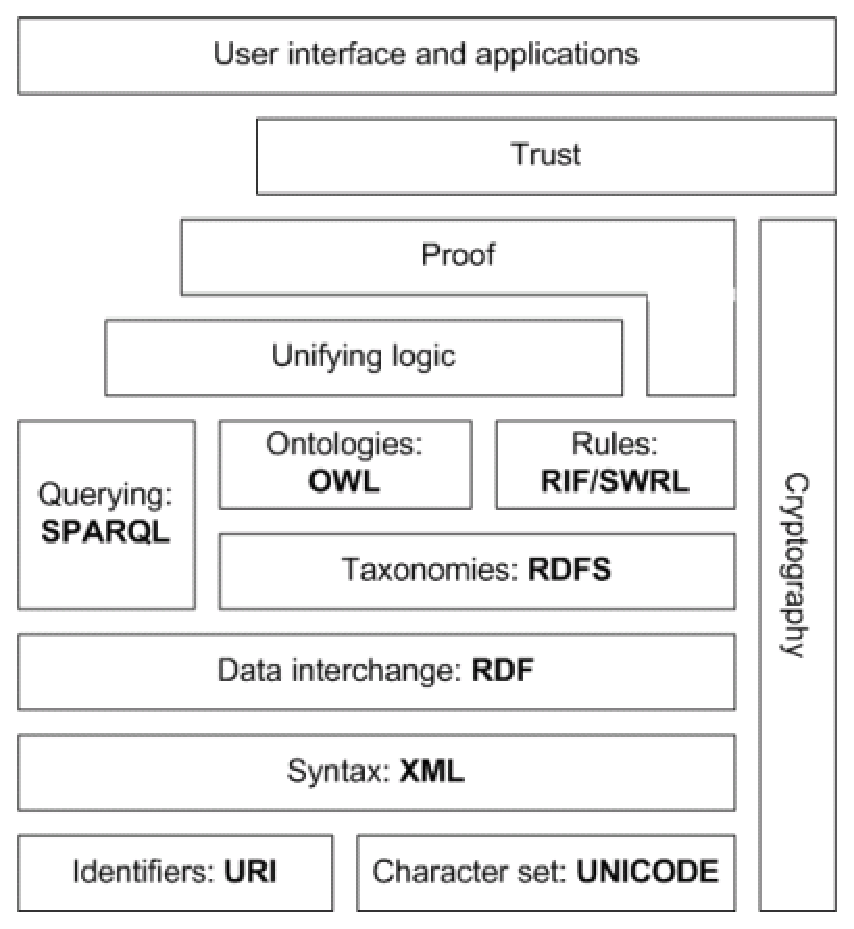
\includegraphics[height=\textheight]{../pics/semantic-web-layers.eps}

\myslide{Semantic Web Architecture (details)}
\begin{itemize}
\item Identify things with  \blu{Uniform Resource Identifiers}
  \begin{itemize}
  \item \blu{Universal Resource Name}: \url{urn:isbn:1575864606}
  \item \blu{Universal Resource Locator:}: \url{http://www3.ntu.edu.sg/home/fcbond/}
  \end{itemize}
\item Identify relations with  \blu{Resource Description Framework}
  \begin{itemize}
  \item Triples of $<$subject, predicate, object$>$
  \item Each element is a \emp{URI}
  \item RDFs are written in well defined XML
  \item You can say anything about anything
  \end{itemize}
\item You can build relations in ontologies (\blu{OWL})
  \begin{itemize}
  \item Then reason over them, search them, \ldots
  \end{itemize}
\end{itemize}


\myslide{Overview of Citation, Reputation and PageRank}

\begin{itemize}
\item Citation and Reputation
  \begin{itemize}
  \item Identifying high quality research
  \end{itemize}
\item PageRank (Google's algorithm for ranking web pages)
  \begin{itemize}
  \item Identifying interesting web pages
  \end{itemize}
\end{itemize}

\myslide{Citation Networks}

\begin{itemize}
\item How can we tell what is a good scientific paper?
  \begin{itemize}
    \item Content-based
    \begin{itemize}
    \item Read it and see if it is interesting (hard for a computer)
    \item Compare it to other things you have read and liked
    \end{itemize}
  \item     Context based 
    \begin{itemize}
    \item See who else read and thought it interesting enough to cite
    \end{itemize}
  \end{itemize}
\end{itemize}
\myslide{Citation Networks}

\begin{itemize}
\item Citation networks are information networks formed by citations
  between articles. Citation networks arise from scientific
  publications, patent filings, or other more exotic information
  systems.
\item Citation networks are directed graphs
  \begin{itemize}
  \item Can be cyclic --- papers can cite each other!
  \end{itemize}

\item Citation networks feature a distinct time-arrow, because researchers can only cite articles that have already been written. As a result, movement on a citation network is always backwards in time.

\item Citations are rarely altered after an article is published. Thus, unlike the www, links in citation networks are never updated. One known consequence of this is that citation networks are prone to serious ageing effects.
\end{itemize}

\myslide{Reputation and Citation Analysis}

\begin{itemize}
\item One major use of citation networks is in measuring productivity
  and impact of the published work of a scientist, scholar or research
  group
\item Some scores are
  \begin{itemize}
  \item Total Number of Citations \hfill (\emp{Pretty Useful})
  \item Total Number of Citations minus Self-citations
  \item Total Number of (Citations / Number of Authors)
  \item Average (Citation * IF / Number of Authors)
  \end{itemize}
\item Problems
  \begin{itemize}
  \item Not all citations are equal: citations by `good' papers are better
  \item Newer publications suffer in relation to older ones
  \item Newer researchers suffer in relation to older ones
  \end{itemize}
\end{itemize}


\myslide{Impact Factor (IF)}

\begin{itemize}
\item (IF) is a measure reflecting the average number of citations to
  articles published in journals
  \begin{quote}
IF(Journal) = the average number of citations received per paper published in that journal during the $n$ preceding years (default $n = 2$)
  \end{quote}
  Depends a lot on finding all the citations
%\item It is used to estimate the relative importance of a journal within its field    

\item It is used to estimate the relative importance of a journal within its field
\item Journals with higher impact factors are more important than those with lower ones.
\end{itemize}

\myslide{Impact Factor (Validity)}

\begin{itemize}
\item The impact factor is highly discipline-dependent
\item The percentage of total citations occurring in the first two years after publication varies highly among disciplines
  \begin{itemize}
  \item 1--3\%  in the mathematical and physical sciences
  \item 5--8\% in the biological sciences
  \end{itemize}
\item In the short term - especially in the case of low-impact-factor journals - many of the citations to a certain article are made in papers written by the author(s) of the original article.
\end{itemize}

\myslide{The Hirsch Index (H-Index)}

\begin{itemize}
\item  Hirsch (2005) writes:

\begin{quote} \itshape{}
  A scientist has index $h$ if $h$ of his/her $N_p$ papers have at least $h$
  citations each, and the other $(N_p - h)$ papers have no more than $h$
  citations each.
\end{quote}
\item In other words, a scholar with an index of $h$ has published $h$ papers
  each of which has been cited in other papers at least $h$ times.
\item Average $h$ differs for different disciplines (and what you count as a citation)
\item In Physics, high $h$ correlates well with whether a scientist has won honors like
  National Academy membership or the Nobel Prize.
\item H-Index is not affected strongly by few papers with many citations and
  many papers with few citations.
\end{itemize}
\newpage

\begin{center}
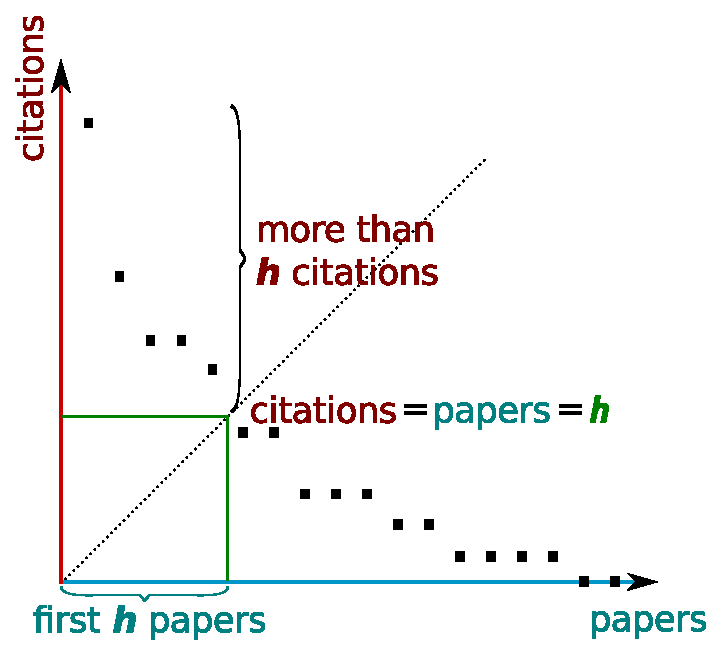
\includegraphics[height=0.9\textheight]{../pics/H-index-en.eps}  
\end{center}



\myslide{Multiple Authors}

\begin{description}\addtolength{\itemsep}{-1ex} 
\item[Natural Sciences] In the life sciences, first listing is usually
  given to the researcher who did most of the work, both physical and
  intellectual, and last billing goes to the mentor or person who
  guided the project and whose grant money paid for the project - the
  PI.
\item[Chemistry] The senior author is sometimes the first author on a
  paper, even if a postdoc completed the bulk of the work.
\item[Archeology, Economics] Strict alphabetical by surname
  \begin{itemize}
  \item Dr Aardvark gets promoted more than Dr Zwilensky
  \end{itemize}
 Liran Einav and Leeat Yariv (2006) ``What's in a Surname? The Effects of Surname Initials on Academic Success'',  
  \textit{The Journal of Economic Perspectives}, \textbf{20(1)}, pp. 175-188
\item Practices also vary by country, \ldots
\end{description}

\myslide{Who to include}
\begin{description}
\item [Honorary Authorship] In many places, the project PI or research
   group leader is always included (even if they have not read the
  paper).  The United States National Academy of Sciences, warns that
  such practices ``dilute the credit due the people who actually did
  the work, inflate the credentials of those so 'honored,' and make
  the proper attribution of credit more difficult.''.

% Honorary authorship is sometimes granted to those who played no significant role in the work, for a variety of reasons. Until recently, it was standard for the head of a German department or institution to be listed as an author on a paper regardless of input.[16] The United States National Academy of Sciences, however, warns that such practices "dilute the credit due the people who actually did the work, inflate the credentials of those so 'honored,' and make the proper attribution of credit more difficult."[4] The extent to which honorary authorship still occurs is not empirically known. However, it is plausible to expect that it is still widespread, because senior scientists leading large research groups can receive much of their reputation from a long publication list and thus have little motivation to give up honorary authorships.


\item [Ghost Authorship] Ghost authorship occurs when an individual
  makes a substantial contribution to the research but is not listed
  as an author.
  \begin{itemize}
  \item Technicians and data gatherers are typically not included.
  \item Some pharmaceutical companies ghost write papers
  \item Many big names have farms of research assistants, who are
    typically not given authorship.
  \end{itemize}
\end{description}  
% Ghost authorship has been linked to partnerships between industry and higher education. Two-thirds of industry-initiated randomized trials may have evidence of ghost authorship.[18] Ghost authorship is considered problematic especially because it may be used to obscure the participation of researchers with conflicts of interest.[19]

% Litigation against the pharmaceutical company, Merck over health concerns related to use of their drug, Rofecoxib (brand name Vioxx), revealed explicit examples of ghost authorship.[20] Merck routinely prepared journal manuscripts and subsequently recruited external, academically affiliated researchers to be the authors.

% Authors are sometimes included in a list without their permission.[21] Even if this is done with the benign intention to acknowledge some contributions, it is problematic since authors carry responsibility for correctness and thus need to have the opportunity to check the manuscript and possibly demand changes.


\myslide{Gaming Citations}

\begin{itemize}
\item Least/Minimum Publishable Unit
  \begin{itemize}
  \item Break research into small chunks to  increase the number of citations
  \item Sometimes there is very little new information
  \end{itemize}
\item Self citation, in-group citation
\item Write only proceedings (some journals are not often read)
\item Submitting only to High Impact factor journals
\end{itemize}

\begin{center}
  You improve what gets measured 
  \\  not necessarily what you want to improve
\end{center}

\myslide{Judging Citations}

\begin{itemize}
\item Not all citations are positive:
  \begin{itemize}
  \item Contrary to \ul{Bond \textit{et al} (2005)}, we found \ldots
  \item This invalidates \ul{Bond \textit{et al} (2005)}.
  \end{itemize}
\item Not all citations are equal:
  \begin{itemize}
  \item We follow closely \ul{Bond \textit{et al} (2005)} as it is efficient and accurate.
  \item Other approaches include \ul{Band \textit{et al} (2004); Bind (2006); Bend (2000)}.
  \end{itemize}
\item Recent research tries to classify the citation types using cue phrases:
  \begin{itemize}
  \item Statement of weakness
  \item Contrast or comparison
  \item Agreement/Usage
  \item Neutral 
  \end{itemize}
\end{itemize}

\myslide{Other uses of Citation NetWorks}
\begin{itemize}
\item Measure the similarity of two articles by the overlap
  of other articles citing them.
\item This is called \blu{co-citation similarity}.
%%% FIXME ADD SLIDE
\\ Two ways of measuring similarity based on hyperlinks:
\begin{itemize}
\item Cocitation similarity: The two articles are cited by the
  same articles.
\item Bibliographic coupling similarity: The two articles
  cite the
  same articles.
\end{itemize}
\item Co-citation similarity on the web: Google's ``find
  pages like this'' or ``Similar'' feature
\item Citation analysis is a big deal: The budget and salary
  of this lecturer are / will be determined by the impact of
  his publications!
\end{itemize}

\myslide{How do you decide what to cite?}



\myslide{Ranking Web Pages}


\begin{itemize}
\item Static Ranking
\item Page Rank
\item Gaming Rankings
\item Digital Object Identifier (DOI)
\end{itemize}



\myslide{Static Ranking}
\begin{itemize}
\item Known Reputable  Sites
\begin{itemize}
\item Wikipedia, \url{.edu} domains, \ldots
\end{itemize}
\item  Spam detection
\item (Real) Popularity (number of click throughs in search)
\item  Page features
  \begin{itemize}
  \item Length of page, length of URL
  \end{itemize}
\item Anchor Text features
\begin{itemize}
\item How much text in links to page, how varied,  \ldots 
\end{itemize}
\end{itemize}


\myslide{Ranking Web Pages}

\begin{itemize}
\item \blu{Web Characteristics}: What does the web look like

\item \blu{Anchor text}: What exactly are links on the web and why are
  they important for finding web pages?

\item \blu{Citation analysis}: the mathematical foundation of
  PageRank and link-based ranking

\item \blu{PageRank}: the original algorithm that was used by Google for
  link-based ranking on the web

\item \blu{Gaming PageRank}: Search Engine Optimization

\item Other Applications

\end{itemize}

\myslide{Characteristics of the Web: Graph}
\MyLogo{Manning, Raghavan and Schütze (2008)}

\begin{center}
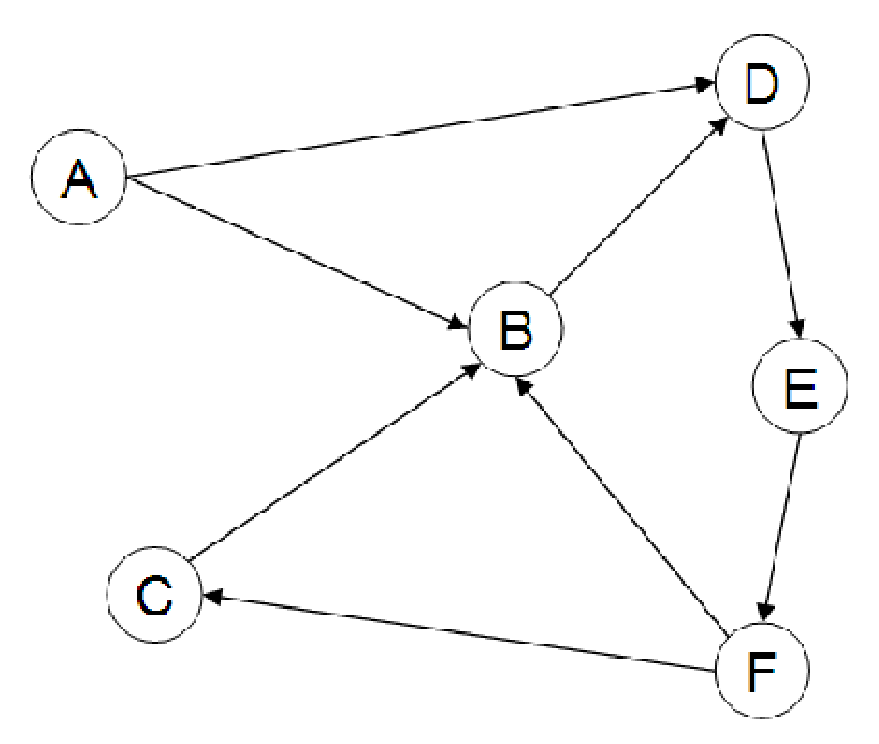
\includegraphics[height=0.8\textheight]{../pics/graph.eps}  
\end{center}

You can't go anywhere from anywhere!

\myslide{Characteristics of the Web: Bow Tie}

\begin{center}
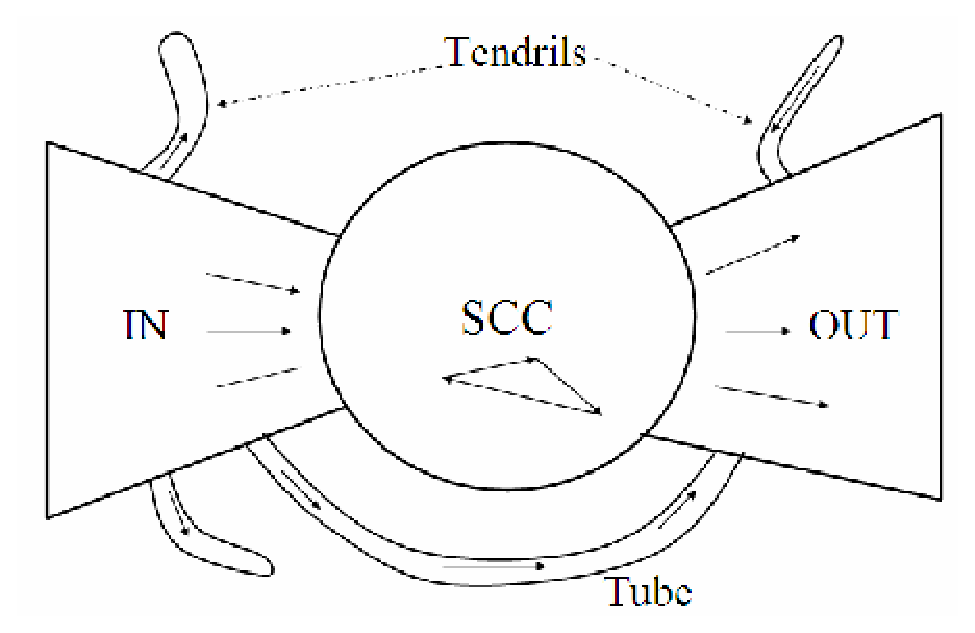
\includegraphics[height=0.8\textheight]{../pics/web-bowtie-bw.eps}  
\end{center}
\blu{SCC}: Strongly Connected Core --- can travel from any page to any page


\myslide{Anchor Text}

\begin{itemize}
\item Recall how hyperlinks are written: \vspace{-1ex}
\begin{verbatim}
<a href="http://path.to.there/page/HG803/">HG803: 
Language, Technology and the Internet.</a>
\end{verbatim}
\begin{verbatim}
For more information about Language, Technology and the
Internet, see the <a href="http://..">HG803 Course Page.</a>
\end{verbatim}
\item Link analysis builds on two intuitions:
  \begin{enumerate}
  \item The hyperlink from A to B represents an endorsement of page B, by the creator of page A.

  \item The (extended) anchor text pointing to page B is a good description of page B.
  \end{enumerate}
  \small {This is not always the case; for instance, most corporate websites have a pointer from every page to a page containing a copyright notice.}
\end{itemize}






%\section{Anchor text}

\myslide{The web as a directed graph}

\psset{unit=8mm}
\begin{small}
  % \fbox{
  \begin{pspicture}(0,-1.5)(12,3.8)

    % \rput(5,1){\circlenode{A}{page $d_1$ \parbox{1cm}{}}}
    \rput(5,1){\circlenode{A}{\makebox[6em]{page $d_1$}}}
    \rput(5,0){\rnode{H}{\blu{\ul{anchor text}}}}
    \rput(12,1){\circlenode{B}{\makebox[6em]{page $d_2$}}}
    \ncline[nodesep=0pt]{->}{H}{B}
    % \Aput{hyperlink}

  \end{pspicture}
  % % }
\end{small}


\begin{itemize}
\item {Assumption 1: \blu{A hyperlink is a quality
 signal.}}
\begin{itemize}
\item {Hyperlink $d_1 \rightarrow d_2$ implies that
  $d_1$'s author deems $d_2$ high-quality and relevant.}
\end{itemize}
\item {Assumption 2: \blu{The anchor text
    describes the content of
  $d_2$.} }
\begin{itemize}
\item {We use anchor text loosely here for any text surrounding the hyperlink. }
\item {Example: ``You can find cheap
  cars $<$a href=http://...$>$here$<$/a$>$.''}
\item {Anchor text: ``You can find cheap
  cars here''}
\end{itemize}
%\item {Easy to find cases where these two
%  assumptions are violated.}
%\item {But they hold for most hyperlinks.}
\end{itemize}

\myslide{[text of $d_2$] only vs.\ [text of $d_2$] + [anchor text $\rightarrow d_2$]}

\begin{itemize}
\item  Searching on [text of $d_2$] +
    [anchor text $\rightarrow d_2$] is often more effective than
  searching on [text of $d_2$] only.
\item Example: Query \emph{IBM}
\begin{itemize}
\item Matches IBM's copyright page
\item Matches many spam pages
\item Matches IBM wikipedia article
\item May not match IBM home page!
\item  \ldots if IBM home page is mostly graphics
\end{itemize}
\item Searching on [anchor text $\rightarrow d_2$] is better for the query \emph{IBM}.
\begin{itemize}
\item In this representation, the page with the most
  occurrences of \emph{IBM} is www.ibm.com.
\end{itemize}
\end{itemize}

\myslide{Anchor text containing \emph{IBM} pointing to www.ibm.com}

\psset{unit=5mm}

\begin{pspicture}(-7,0)(30,20)



\rput(5,18){www.nytimes.com: ``\rnode{A}{IBM} acquires Webify''}
\rput(10,13){www.slashdot.org: ``New \rnode{B}{IBM}
  optical chip''}
\rput(15,8){www.stanford.edu: ``\rnode{C}{IBM}
  faculty award recipients''}
\rput(10,2){\rnode{D}{\psframebox{wwww.ibm.com}}}

{
\ncline[nodesep=3pt,linestyle=dashed]{->}{A}{D}
\ncline[nodesep=3pt,linestyle=dashed]{->}{B}{D}
\ncline[nodesep=3pt,linestyle=dashed]{->}{C}{D}
}

\end{pspicture}






% \myslide{Indexing anchor text}

% \begin{itemize}
% \item Thus: Anchor text is often a better description of a
%   page's content than the page itself.
% \item Anchor text can be weighted more highly than document
%   text. (based on Assumptions 1\&2)
% %\item Indexing anchor text can have undesirable side
% %  effects -- \blu{Google bombs}.
% \end{itemize}


\myslide{Exercise: Assumptions underlying PageRank}

\begin{itemize}
\item Assumption 1: A link on the web is a quality signal --
  the author of the link thinks that the linked-to page is
  high-quality.
\item Assumption 2: The anchor text describes the content of
  the linked-to page.
\item Is assumption 1 true in general?
\item Is assumption 2 true in general?
\end{itemize}



\myslide{Google bombs}

\begin{itemize}
\item A Google bomb is a search with ``bad'' results due to
maliciously manipulated  anchor text.
\item Google introduced a new weighting function
in January 2007
that fixed many Google bombs.
%\item An ``msn bomb''
% (2007.06.29):
%\url{http://search.msn.co.uk/results.aspx?q=liar}
\item Still some remnants: [dangerous cult] on Google,
  Bing, Yahoo
\begin{itemize}
\item Coordinated link creation by those who dislike the
  Church of Scientology
\end{itemize}
\item Defused Google bombs: [dumb motherf....], [who is a
  failure?], [evil empire]
\end{itemize}



%\section{Citation analysis}

\myslide{Origins of PageRank: Citation analysis (1)}

\begin{itemize}
\item \blu{Citation analysis}: analysis of citations in the scientific literature
\item Example citation: ``\blu{Miller (2001)} has shown that physical
  activity alters the metabolism of estrogens.''
\item We can view ``Miller (2001)'' as a hyperlink linking two
  scientific articles.
\item One application of these ``hyperlinks'' in the
  scientific literature:
\end{itemize}


\myslide{Origins of PageRank: Citation analysis (2)}

\begin{itemize}
\item Another application: Citation frequency can be used to measure
  the \blu{impact} of an article.
\begin{itemize}
\item Simplest measure: Each article gets one vote -- not
  very accurate.
\end{itemize}
\item On the web: citation frequency = \blu{inlink count}
\begin{itemize}
\item A high inlink count does not necessarily
  mean high quality \ldots
\item \ldots mainly because of link spam.
\end{itemize}
\item Better measure: \blu{weighted} citation frequency or citation rank
\begin{itemize}
\item An article's vote is weighted according to its
  citation impact. 
\item Circular? No: can be formalized in a
  well-defined way.
\end{itemize}
\end{itemize}


\myslide{Origins of PageRank: Citation analysis (3)}

\begin{itemize}
\item \blu{PageRank}: weighted citation frequency or citation rank
\item PageRank was invented in the context of citation
  analysis by \citet{PINSKI1976297} in the 1970s.
\end{itemize}



\myslide{Origins of PageRank: Summary}

\begin{itemize}
\item We can use the same formal representation for
\begin{itemize}
\item citations in the scientific literature
\item hyperlinks on the web
\end{itemize}
\item Appropriately weighted citation frequency is an
  excellent measure of  quality \ldots
\begin{itemize}
\item \ldots both for web pages and for scientific publications.
\end{itemize}
\item Next: PageRank algorithm for computing weighted
  citation frequency on the web
\end{itemize}




%\myslide{Link-based ranking for web search}

%\begin{itemize}
%\item Simple version of using links for ranking on the web
%\begin{itemize}
%\item First retrieve all pages satisfying the query (say
%  \emph{venture capital})
%\item Order these by the number of inlinks
%\end{itemize}
%\item Simple link popularity (= number of inlinks)
%is easy to spam. Why?
%\end{itemize}


%\section{PageRank}

\myslide{Model behind PageRank: Random walk}
\begin{itemize}
\item Imagine a web surfer doing a random walk on the web \com{virtual}
\begin{itemize}
\item Start at a random page
\item At each step, go out of the current page along one of
  the links on that page, equiprobably
\end{itemize}
\item In the steady state, each page has a \blu{long-term visit rate}.
  \\ what proportion of the time someone will be there
\item This long-term visit rate is the page's \blu{PageRank}.
\item \blu{PageRank 
=
  long-term visit rate
\\ = steady state probability of being at a page
}
\end{itemize}



\myslide{Long-term visit rate}

\begin{itemize}
\item Recall: PageRank = long-term visit rate
\item Long-term visit rate of page $d$ is the probability that a web surfer
  is at page $d$ at a given point in time.
\item To calculate this the web graph must not contain
  \blu{dead ends}.
  \begin{itemize}
  \item But the web is full of dead ends
  \item Random walk can get stuck in dead ends
  \item If there are dead ends, long-term visit
    rates are not well-defined (or non-sensical)
  \end{itemize}
  \end{itemize}


\myslide{Teleporting -- to get us out of dead ends}
\begin{itemize}
\item At a \blu{dead end}, jump to a random web page with
  prob.\ $1/N$.
\item At a \blu{non-dead end}, with probability 10\%, jump to a
  random web page (to each with a probability of $0.1/N$).
\item With remaining probability (0.9), go out on a random
  hyperlink.
\begin{itemize}
 \item For example, if the page has 4 outgoing links:
   randomly choose one with probability (1-0.10)/4=0.225
\end{itemize}
\item 10\% is a parameter, the \blu{teleportation rate}.
\item Note: ``jumping'' from a dead end is
independent of teleportation rate.
\end{itemize}

% \myslide{Result of teleporting}
% \begin{itemize}
% \item With teleporting, we cannot get stuck in a dead end.
% \item But even without dead ends, a graph may not have
%   well-defined long-term visit rates.
% \end{itemize}

\myslide{How do we compute the steady state vector?}
\begin{itemize}
\item In other words: how do we compute PageRank?
\item Recall:  $\vec{\pi} = (\pi_1,\pi_2,\ldots,\pi_N)$
is the PageRank vector, the vector of steady-state probabilities \ldots
\item \ldots and if the distribution in this step is 
 $\vec{x}$, then the distribution in the next step is
  $\vec{x} P$.
\item But $\vec{\pi}$ is the steady state: $\vec{\pi} = \vec{\pi} P$
\item Solving this matrix equation gives us $\vec{\pi}$.
\item $\vec{\pi}$ is the principal left eigenvector for $P$ 
  \\ (a well known mathematical concept)
\end{itemize}


\myslide{One way of computing the PageRank $\vec{\pi}$}
\begin{itemize}
\item Start with any distribution $\vec{x}$, e.g., uniform distribution
\item After one step, we're at $\vec{x} P$.
\item After two steps, we're at $\vec{x} P^2$.
\item After $k$ steps, we're at $\vec{x} P^k$.
\item Algorithm: multiply $\vec{x}$ by increasing powers of $P$
  until convergence.
\item This is called the \blu{power method}.
\item Regardless of where we start, we eventually reach the steady state $\vec{\pi}$.
\item Thus: we will eventually (in asymptotia) reach the steady state.
\end{itemize}

\myslide{Example Graph}
\MyLogo{http://www.ams.org/samplings/feature-column/fcarc-pagerank}
\begin{center}
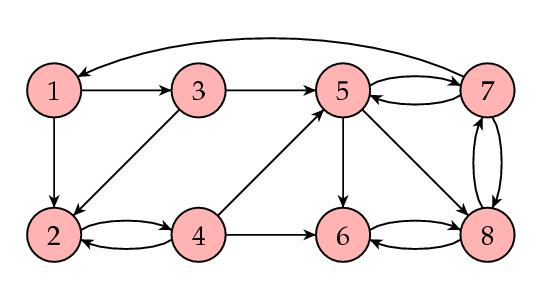
\includegraphics[height=0.8\textheight]{../pics/goodnet.jpg}  
\end{center}
Each inbound link is a positive vote.


\myslide{Example Graph: Weighted}
\begin{center}
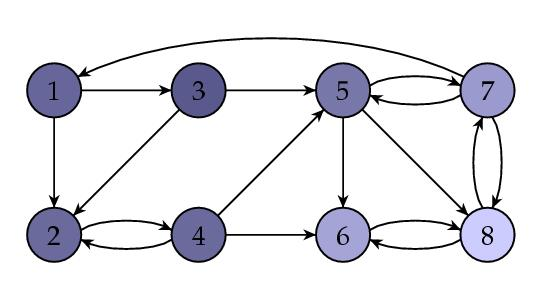
\includegraphics[height=0.8\textheight]{../pics/goodnet-shaded.jpg}  
\end{center}

Pages with higher PageRanks are lighter. 


\myslide{PageRank summary}
\MyLogo{}
\begin{itemize}
\item Preprocessing
\begin{itemize}
\item Given graph of links, build matrix $P$
\item Apply teleportation
\item From modified matrix, compute $\vec{\pi}$
\item $\vec{\pi}_i$ is the PageRank of page $i$.
\end{itemize}
\item Query processing
\begin{itemize}
\item  Retrieve pages satisfying the query
\item Rank them by their PageRank
\item Return reranked list to the user
%\item Note: this ranking is query-\blu{independent}.
%\item Problematic in  cases like \emph{video service}
\end{itemize}
\end{itemize}

\myslide{PageRank issues}
\begin{itemize}
\item Real surfers are not random surfers.
\begin{itemize}
\item Examples of nonrandom surfing:
  \begin{itemize}
  \item back button
  \item short vs.\ long paths
  \item bookmarks
  \item directories
  \item search!
  \end{itemize}
\item [$\Rightarrow$] \txx{Markov model} 
  (future states depend only on the present state) is
  not a good model of surfing.
\item But it's good enough as a model for our purposes.
\end{itemize}
\newpage
\item Simple PageRank ranking  produces bad results for many
  pages.  
\begin{itemize}
\item Consider the query \txx{[video service]}
\item The Yahoo home page (i) has a very high PageRank and (ii)
  contains both \emph{video} and \emph{service}.
\item If we rank all Boolean hits according to PageRank,
  then the Yahoo home page would be top-ranked.
\item Clearly not desirable
\end{itemize}
\item In practice: rank according to weighted combination of
 raw text match, anchor text match,
  PageRank \& other factors
\end{itemize}




\myslide{How important is PageRank?}

\begin{itemize}
\item Frequent claim: PageRank is the most important
  component of web ranking.
\item The reality: 
\begin{itemize}
\item There are several components that are at least as
  important:
  \begin{itemize}
  \item  anchor text
  \item phrases
  \item proximity
  \item tiered indexes
  \end{itemize}
\item Rumor has it that PageRank in its original form (as
  presented here) now has a negligible impact on ranking!
\item However, variants of a page's PageRank are still an
  essential part of ranking.
\item Adressing link spam is difficult and crucial.
\end{itemize}
\end{itemize}


\myslide{Gaming PageRank}

\begin{itemize}
\item \blu{Link Spam} adding links between pages for reasons other
  than merit.  Link spam takes advantage of link-based ranking
  algorithms, which gives websites higher rankings the more other
  highly ranked websites link to it.  Examples include adding links
  within blogs.
\item \blu{Link Farms} creating tightly-knit communities of pages
  referencing each other, also known humorously as mutual admiration
  societies.
\item \blu{Scraper Sites}  "scrape" search-engine results pages or other sources of content and create "content" for a website. The specific presentation of content on these sites is unique, but is merely an amalgamation of content taken from other sources, often without permission.
\newpage
\item \blu{Comment spam} is a form of link spam in web pages that
  allow dynamic user editing such as wikis, blogs, and guestbooks.
  Agents can be written that automatically randomly select a user
  edited web page, such as a Wikipedia article, and add spamming
  links.
\end{itemize}

\begin{itemize}
\item The \blu{nofollow} link: a value that can be assigned to the rel
attribute of an HTML hyperlink to instruct some search engines that a
hyperlink should not influence the link target's ranking in the search
engine's index.
\item Google does not index the target of a link marked \textbf{nofollow}.
\item Yahoo! does not include the link in its ranking
\item \ldots
\end{itemize}


% \myslide{Other Weighting Factors}

%     * Title
%     * Anchor Text
%     * Font/Color
%     * Position on page
%     * Implicit Feedback 

\myslide{Search Engine Optimization}

\begin{itemize}
\item \blu{Search engine optimization (SEO)} is the process of
  improving the visibility of a web site or a web page in search
  engines.
  \begin{itemize}
  \item Getting Indexed
  \item Cross Linking
  \item URL normalization
  \item Meta Tags
  \item Paid Links (AdSense)
  \end{itemize}
\item The ultimate method:
  \begin{itemize}
  \item Writing interesting pages with content people want to read 
  \end{itemize}
\end{itemize}

\myslide{Current Status}

\begin{itemize}
\item There is a continuous battle between 
  \begin{itemize}
  \item Search companies, who want to get the most useful page to the user
  \item Page writers, who want to get their page read
  \end{itemize}
\item \emp{All metrics get gamed}
\end{itemize}

% \myslide{Google Scholar}

\myslide{Improving Citation Networks}

\begin{itemize}
\item When most scholarship was in journals or books, then citation was easy
\\ or at least bounded 
\begin{itemize}
\item[\Bad] Although in reality most people could access few resources
\end{itemize}
\item Now many papers or sources of information only exist online or as files.
\item Things on line move around, which makes citations unreliable
\item We need \txx{Persistent Identifiers}
  \begin{itemize}
  \item \txx{Uniform Resource Name (URN)}
    \begin{itemize}
    \item ISBN
    \item Archived Web Pages
    \end{itemize}
  \item \txx{Digital object identifier (DOI)}
  \end{itemize}
\end{itemize}

\myslide{Digital object identifier}
\begin{itemize}
\item \blu{DOI}: a string used to uniquely identify an electronic document or object
\item Metadata  about the object is stored with the DOI name
\item The metadata includes a location, such as a URL
\item The DOI for a document is permanent, whereas the metadata may change
\item Thus the DOI provides more stable linking than URLs
\item  The DOI system is implemented through a federation of registration agencies coordinated by the International DOI Foundation
\item By late 2009 approximately 43 million DOI names had been assigned by some 4,000 organizations
  \begin{itemize}
  \item 100 millionth DOI assigned in 2014
  \item  10 millionth DOI  assigned in August 2003
  \item  millionth DOI was assigned in April 2000
  \end{itemize}
\end{itemize}

\myslide{DOI example}

\begin{itemize}
\item DOI: \emp{10.1007/s10579-008-9062-z} has metadata
\begin{verbatim}
url = http://www.springerlink.com/content/v7q114033401th5u/
type = journal 
last1 = Bond | first1 = F. 
last2 = Fujita | first2 = S. 
last3 = Tanaka | first3 = T. 
title = The Hinoki syntactic and semantic treebank of Japanese 
journal = Language Resources and Evaluation 
volume = 42 
pages = 243 
year = 2008 
\end{verbatim}
\end{itemize}

\myslide{DOI characteristics}

\begin{itemize}
\item An ID backed by 
\begin{itemize}
\item Persistence, if material is moved, rearranged, or bookmarked
\item Interoperability with other data from other sources
\item Extensibility by adding new features and services through management of groups of DOI names
\item Single management of data for multiple output formats
\item Class management of applications and services
\item Dynamic updating of metadata, applications and services
\end{itemize}
\end{itemize}

Makes it easier to correctly count citations -- makes analysis more reliable


% \myslide{Summary}

% \myslide{Pagerank}

% Direct application of Pagerank to citation networks captures the relative importance of citing papers in a manner that is self-consistent. However, because citations cannot be updated after publication, links in citation networks may not represent an up-to-date reflection of relevancy. For an older publication that is not likely to receive any new citations, this is of little consequence. For this reason, the Pagerank of such a publication may be interpreted as its lifetime achievement award. For recent publications, however, the interpretation is not so clear.

% Traffic flows along citation links, traveling backwards through time to older papers. Pagerank distributes initial traffic equally across the network. A recent paper therefore has a significantly lower proportion of incoming traffic, due to the smaller number of papers published afterwards.

% The assumption, implicit to Pagerank, that traffic distribution is blind to the age of publications is not valid for citation networks. After all, scientific research is time-critical and often builds upon recent progress. Researchers do not usually begin their search by looking at age-old publications, so why model them that way?
% CiteRank

% The most appropriate ranking method incorporates a more believable traffic distribution for researchers exploring the citation network. A random researcher selects a recent paper with probability that exponentially decreases according to the age of the publication. With a certain probability, the researcher randomly follows one of the citations to the next paper, and so forth.





\myslide{Other networks you can analyse}

\begin{itemize}
\item Disease transfer --- who infected whom
\item Social networks --- who friended whom 
  \\ Kevin Bacon game
 % IT crowd
\item Semantic Networks 
%  \\ FIXME: Dominic
\end{itemize}

\myslide{Summary of PageRank}
\MyLogo{}
\begin{itemize}
\item Given a graph, ranks nodes according to their relative structural
  importance
  \begin{itemize}
  \item If an edge from $n_i$ to $n_j$ exists, a vote from $n_i$ to $n_j$ is produced
  \item Strength depends on the rank of $n_i$
  \item The more important  $n_i$ is, the more strength its votes will have.
  \end{itemize}
\item PageRank can also be viewed as the result of a random walk process
  \begin{itemize}
  \item Rank of  $n_i$ represents the probability of a random walk over the graph ending
    on  $n_i$, at a sufficiently large time.
  \end{itemize}
\end{itemize}

% \myslide{Summary}

% \begin{itemize}
% \item 
% \end{itemize}

\myslide{Fake News}

\begin{itemize}
\item Fake news is \emp{false} news
  \begin{itemize}
  \item Malicously False News
  \item Satire
  \item Disinformation
  \item Misinformation
  \item Rumour
  \end{itemize}
\item Fake news is \emp{intentionally} and \emp{verifiably} false news
  \emp{published by a news outlet}
\end{itemize}




\myslide{Acknowledgments and Further Reading}

\begin{itemize}
\item Excellent introduction to Information Retrieval, including web searching:
\\ Christopher D. Manning, Prabhakar Raghavan and Hinrich Schütze, \textit{Introduction to Information Retrieval}, Cambridge University Press. 2008. 
\\ \url{http://nlp.stanford.edu/IR-book/information-retrieval-book.html}
\item David Austin (2010) \textit{How Google Finds Your Needle in the Web's Haystack}
American Mathematical Society, Monthly Column 
\\ \url{http://www.ams.org/samplings/feature-column/fcarc-pagerank}
%\item Citerank \url{http://www.cmth.bnl.gov/~maslov/citerank/}
\item Hirsch, J. E. (2005). "An index to quantify an individual's scientific research output". \textit{Proceedings of the National Academy of Science} \textbf{102(46)}: 16569–16572. 
\item Gabriel Pinski, Francis Narin (1976)
\href{https://doi.org/10.1016/0306-4573(76)90048-0}{Citation influence for journal aggregates of scientific publications: Theory, with application to the literature of physics},
\textit{Information Processing \& Management},
\textbf{12:5}  pp 297-312, ISSN 0306-4573.

\item Xinyi Zhou, Reza Zafarani \href{https://arxiv.org/abs/1812.00315}{Fake News: A Survey of Research, Detection Methods, and Opportunities} arxiv.org, retrieved 2019-04-03
\item Olga Yurkova (2018) \href{https://gijn.org/six-fake-news-techniques-and-simple-tools-to-vet-them/}{Six Fake News Techniques and Simple Tools to Vet Them} Global Investigative Journalism Network, accessed 2019-04-03} [mainly non-linguistic methods]
\item  Hannah Rashkin, Eunsol Choi, Jin Yea Jang, Svitlana Volkova and Yejin Choi (2017) \href{https://www.aclweb.org/anthology/D17-1317/}{Truth of Varying Shades: Analyzing Language in Fake News and Political Fact-Checking} Proceedings of the 2017 Conference on Empirical Methods in Natural Language Processing, pages 2931–2937 Copenhagen, Denmark, September 7–11, 2017. c 2017 Association for Computational Linguistics

\end{itemize}
\end{document}


%%% Local Variables: 
%%% coding: utf-8
%%% mode: latex
%%% TeX-PDF-mode: t
%%% TeX-engine: xetex
%%% End: 

